\documentclass[article]{repec}
\usepackage{amsmath,amssymb,rotating,multirow,thumbpdf}
\graphicspath{{graph/}}

\author{Marcin Błażejowski\\WSB University in Toruń\ \And
        Jacek Kwiatkowski\\Nicolaus Copernicus University in Toruń}
\Plainauthor{Marcin Błażejowski, Jacek Kwiatkowski}

\title{Bayesian Model Averaging and Jointness Measures for \pkg{gretl} -- 2.1}
\Plaintitle{Bayesian Model Averaging and Jointness Measures for gretl -- 2.1}

\Abstract{Bayesian model averaging is a model-building strategy that
  takes account of model uncertainty in
  conclusions about estimated parameters. It is an efficient tool for
  discovering the most probable models and obtaining estimates of
  their posterior characteristics. We introduce
  the \pkg{BMA} package for linear regression models with jointness measures
  proposed by \cite{LeySteel2007} and \cite{DoppelhoferWeeks2009}.
  More information one can find in \cite{Blazejowski_Kwiatkowski_BMA_JSS}.}

\Keywords{Bayesian model averaging, jointness measures, \pkg{gretl}, \proglang{Hansl}}
\Plainkeywords{Bayesian model averaging, jointness measures, gretl, Hansl}

\Address{
  Marcin Błażejowski\\
  Department of Quantitative Methods\\
  WSB University in Toruń\\
  87-100 Toruń, Poland\\
  E-mail: \email{marcin.blazejowski@wsb.torun.pl}\\

  Jacek Kwiatkowski\\
  Department of Econometrics and Statistics\\
  Faculty of Economics and Management\\
  Nicolaus Copernicus University in Toruń\\
  87-100 Toruń, Poland\\
  E-mail: \email{jkwiat@umk.pl}
}

\begin{document}
	
\section*{Changelog}
\begin{description}
	\item[2.1] Small code refreshing:
		\begin{itemize}
			\item Some code cleanups.
			\item Getting rid of calls to deprecated functions.
			\item Correct handling of missing values.
		\end{itemize}
	\item[2.0] Bundle based version (most of internal
		functions call only \texttt{bundle M}).
	\item[1.0] Initial version.
\end{description}

\section{Introduction}\label{BmaGretlSec1}
We know from elementary statistical theory that linear regression
attempts to model the relationship between two or more variables by
fitting a simple linear equation to observed data. In the classical
approach, we usually rely on ordinary least squares (OLS) or maximum
likelihood (ML) estimates and popular model selection criteria, i.e.,
the Akaike information criterion (AIC) and the Bayesian information
criterion (BIC), to find the ``best'' model. A problem with this
approach arises when we have to select a ``good'' subset of variables
from a large set of regressors. When the number of possible exogenous
variables is $K$, the number of possible linear models is $2^K$.  If
we have, for example, $K=30$ possible regressors, the number of
possible combinations of variables to be included or not equals
1073741824. This means that it is very difficult, if not impossible,
to find the estimates for all combinations. Moreover,
\cite{RafteryMadiganHoeting1997} show that standard variable selection
procedures lead to different estimates and conflicting conclusions
about the main questions of interest.

Bayesian model averaging is a useful alternative to other variable
selection procedures, because it incorporates model uncertainty into
conclusions about the estimated parameters.  Bayesian model averaging
is a standard Bayesian solution to model uncertainty, where the
inference on parameters is based on a weighted average over all
possible models under consideration, rather than on one single
regression model. These weights are the Bayesian posterior
probabilities of the individual models.

There is a recent and growing literature on Bayesian model
averaging. Examples of applications of Bayesian model averaging can be
found in a number of works (see, for example,
\citealt{HoetingMadiganRafteryVolinsky1999}, \citealt{Steel2011} for a
recent overview).  Our software package for parameter estimation and
model comparison of linear regression models is based on
\cite{FernandezLeySteel2001a,FernandezLeySteel2001b} and
\cite{Koop2003}. We use the Markov chain Monte Carlo model composition
($\mbox{MC}^3$) sampling algorithm developed by \cite{MadiganYork1995}
to select a representative subset of models.

\cite{DoppelhoferWeeks2005,DoppelhoferWeeks2009} define a jointness
measure of dependence among explanatory variables that appear in the
linear regression models. We use this measure to identify whether two
variables are substitutes, complements or neither.  A similar
jointness measure was also proposed by \cite{LeySteel2007}.

In this paper, we propose Bayesian model averaging package for
\pkg{gretl}, \citep{gretl} named \pkg{BMA}.  We can list several reasons
why, in our opinion, it is important to address this topic. \pkg{gretl} is
an increasingly popular, free, open-source software for econometric
analysis, both for students and academics. It is written in pure
\proglang{C} ``by econometricians for econometricians'' with the
international community gathered around two men: Allin Cottrell and
Riccardo ``Jack'' Lucchetti. Since 2009 the community has been meeting
every two years at the \pkg{gretl} conference. The last conference was held
in Berlin on June 12--13, 2015.  \pkg{gretl} is licensed under the GPL-3
license (\url{http://www.gnu.org/copyleft/gpl.html})  and has been reviewed
several times in various international journals.  The best known
reviews were written by
\cite{RePEc:jae:japmet:v:18:y:2003:i:1:p:105-110},
\cite{RePEc:jae:japmet:v:22:y:2007:i:4:p:849-854} and
\cite{Rosenblad:2008:JSSOBK:v25s01}. Some brief information about
\pkg{gretl} was also presented in \cite{Lucchetti:2010:JSSOBK:v41i11} and
\cite{RePEc:wly:japmet:v:26:y:2011:i:5:p:880-885}.  Unlike most other
statistical software packages \pkg{gretl} has an easy-to-use graphical user
interface (GUI). Our software package is, therefore, a free and
easy-to-use tool for Bayesian model averaging.

The rest of the paper is organized as follows:
Section~\ref{BmaGretlSec2} briefly outlines Bayesian model averaging
for linear regression models with the $\mbox{MC}^3$ sampling algorithm and
jointness measures.  Section~\ref{BmaGretlSec3} provides an overview
of the \pkg{gretl} packages for Bayesian model averaging.
Section~\ref{BmaGretlSec4} includes an overview of Bayesian model
averaging software packages.  Section~\ref{BmaGretlSec5} presents
an empirical illustration. The final section concludes.


%%%%%%%%%%%%%%%%%%%%%%%%%%%%%%%%%%%%%%%%%%%%%%%%%%%%%%%%%%%%%%%%%%%%%%%%%%%%%%%%%%%%%%%%
\section{Bayesian inference in normal linear regression models}\label{BmaGretlSec2}
In this section, we briefly introduce the main features of Bayesian
inference in linear regression models. We present Bayesian estimation
and prediction with normal-gamma natural conjugate priors and many
explanatory variables, as well as model selection and Bayesian model
averaging techniques. Finally, in this section we present the basics
of the Markov chain Monte Carlo model composition sampling algorithm and
jointness measures.

\subsection{Bayesian estimation, model selection, and prediction}
Let us consider normal linear regression models which differ in their
explanatory variables (see \citealt{Koop2003} for further details).
Suppose that we have $K$ potential explanatory variables, which means
there are $2^K$ possible models and let $M_r$ for $r=1,\dots, 2^K$
denote the $2^K$ different models under consideration.  Suppose also
that $y_i$ and $x_i$ denote the observed data on the dependent and
explanatory variables for $i=1,\ldots,N$. The observations are placed
in a $(N \times 1)$ vector $y$ and a $(N \times k_r)$ matrix $X_r$
containing the set of regressors included in model $M_r$%
\footnote{We subtract the mean from all regressors as in
  \cite{FernandezLeySteel2001a}.}.  Thus, we can write our model as
\begin{equation*}
  y=\alpha \iota_N + X_r\beta_r + \epsilon,
\end{equation*}
where $\iota_N$ is a $(N \times 1)$ vector of ones, $\beta_r$ is a
$(k_r \times 1)$ vector of unknown parameters, $\epsilon$ is a
$(N \times 1)$ vector of errors which are assumed to be normally
distributed, $\epsilon \sim N(0_N, h^{-1}I_N)$ and \textit{h} is the
error precision, which is defined as $h=\frac{1}{\sigma^2}$.
$N(\mu, \Sigma)$ denotes a normal distribution with mean $\mu$ and
variance ${\Sigma}$.  Following \cite{Koop2003}, the prior for
$\beta_r$ is normally distributed,
\begin{equation*}
  \beta_r \mid h, M_r \sim N \left(0_{k_r}, h^{-1} \left [g X_r^\top X_r  \right]^{-1}  \right),
\end{equation*}
while we use a noninformative prior for the intercept and precision,
\begin{equation*}
  p(\alpha) \propto 1, p(h)\propto \frac {1}{h}.
  \label{eq:prior}
\end{equation*}
The factor of proportionality \textit{g} is part of the so-called
Zellner's g-prior \citep{Zellner1986}. This prior is a convenient way
to specify the prior variance matrix, because it reduces the number of
prior variance parameters and considerably simplifies posterior
computations. The \pkg{gretl} package offers the five most popular
alternative Zellner's g-priors (see \citealt{FernandezLeySteel2001a}
and \citealt{Moral-Benito2010}).

\begin{itemize}\label{text:g-priors}
  \item Unit information prior (g-UIP), recommended by \cite{KassWasserman1995}:
    \begin{equation}
      g = \frac{1}{N}.
      \label{eq:g-UIP}
    \end{equation}
  \item Risk inflation criterion (g-RIC), proposed by \cite{FosterGeorge1994}:
    \begin{equation}
    g = \frac{1}{K^2}.
      \label{eq:g-RIC}
    \end{equation}
  \item Benchmark prior, recommended by \cite{FernandezLeySteel2001a}:
    \begin{equation}
    g = \left\{\begin{array}{ll}
	    \frac{1}{K^2} & \mbox{for $N \le K^2$},\\
	    \frac{1}{N} & \mbox{for $N>K^2$}.\end{array} \right. 
      \label{eq:Benchmark_Prior}
    \end{equation}
  \item g-HQ prior which mimics the Hannan and Quinn criterion, see \cite{FernandezLeySteel2001a}:
    \begin{equation}
      g = \frac{1}{(\text{ln}N)^3}.
      \label{eq:g-HQ}
    \end{equation}
  \item Root of g-UIP, see \cite{FernandezLeySteel2001a}:
     \begin{equation}
      g = \sqrt{\frac{1}{N}}.
      \label{eq:root-g-UIP}
    \end{equation}
\end{itemize}
 
By Bayes' rule, the mean of the posterior distribution of the slope
parameters $\beta_r$, conditional on model $M_r$, can be written as
\begin{equation}
  \E(\beta_r \mid y, M_r)= \left [ \left (1+g  \right ) X^\top_rX_r \right ]^{-1}X^\top_ry.
  \label{eq:posterior_mean}
\end{equation}
It is easy to see that if $g \approx 0$ the mean of the posterior
distribution (see Equation~\ref{eq:posterior_mean}) equals the OLS
estimates. The posterior variance of $\beta_r$, conditional on model
$M_r$, is given by
\begin{equation}
  \VAR \left (\beta_r \mid y, M_r \right)=\frac {Ns^2_r}{N-2}\left [ \left (1+g  \right ) X^\top_rX_r \right ]^{-1},
  \label{eq:posterior_variance2}
\end{equation}
where 
\begin{equation*}
  s^2_r=\frac{\frac{1}{1+g} y^\top P_{W_r}y+\frac{g}{1+g} \left( y-\bar y\iota_N \right)^\top \left( y-\bar y\iota_N \right)}{N}
\end{equation*}
and $P_{W_r}=I_N-W_r \left ( W^\top_rW_r \right )^{-1}W^\top_r$ for $W_r=(\iota_N,X_r)$. 

The marginal data density, conditional on model $M_r$, may be written
as
\begin{equation}
  p(y \mid M_r) \propto \left (\frac{g}{1+g}\right)^{\frac{k_r}{2}}
  \left [  \frac{1}{1+g}y^\top P_{W_r}y + \frac{g}{1+g} \left( y-\bar y\iota_N \right)^\top
  \left( y-\bar y\iota_N \right) \right]^{-\frac{N-1}{2}}.
  \label{eq:marginal_data_density}
\end{equation}

In the Bayesian approach of comparing models, it is considered useful
to employ probabilities to represent the degree of belief associated
with the alternative models. For the normal linear regression models
we can easily test two mutually exclusive (non-nested) and jointly
exhaustive models with different subset of variables.  Using Bayes'
theorem, the posterior odds ratio for a model $M_l$ against model
$M_n$ is given by
\begin{equation}
  \frac{\Prob(M_l \mid y)}{\Prob(M_n \mid y)}=\frac{\Prob(M_l)}{\Prob(M_n)}\frac{p(y \mid M_l)}{p(y \mid M_n)},
  \label{eq:posterior_odds_ratio}
\end{equation}
where $\frac{\Prob(M_l)}{\Prob(M_n)}$ is the prior odds ratio and
$\frac{p(y \mid M_l)}{p(y \mid M_n)}$ is the Bayes factor. If the
ratio $\frac{\Prob(M_l \mid y)}{\Prob(M_n \mid y)}$ is larger than 1,
we can say that the data supports model $M_l$ over model $M_n$. In our
package, we use two popular model priors.
\begin{itemize}\label{misc:priors}
  \item Binomial prior:
    \begin{equation}
      \Prob(M_r)=\theta^{k_r}(1-\theta)^{K-k_r}\; \quad\mathrm{for~} r=1, \dots, 2^K.
      \label{eq:model_prior_binomial}
    \end{equation}    
    Note that for $\theta=0.5$ we have a uniform prior on the model space, i.e., $\Prob(M_r)=2^{-K}$.
  \item Binomial-beta prior (see \citealt{GelmanCarlinSternRubin1997}):
    \begin{equation}
      \Prob(\Xi=k_r)= \frac{\Gamma (K+1)}{\Gamma(k_r+1)\Gamma(K-k_r+1)}\cdot
      \frac{\Gamma(a+k_r)\Gamma(K+b-k_r)}{\Gamma(a+b+k_r)} \cdot \frac{\Gamma(a+b)}{\Gamma(a)\Gamma(b)},
      \label{eq:model_prior_binomial-beta}
    \end{equation}
    where $\Xi$ denotes model size. 
\end{itemize}

In our package, we only need to specify the prior expected model size
$\E(\Xi) \in \left (0, K \right ]$.  Note that in case of the binomial
prior we have $\E(\Xi)=K\theta$ and the choice of $\E(\Xi)$
automatically produces a value for the prior inclusion probability
$\theta$. If we have the binomial-beta prior, the average model size
will satisfy $\E(\Xi)=\frac {a}{a+b}K$. Here, we follow
\cite{Ley_Steel_jae_2009} and fix $a=1$ hence obtaining the value of
the second hyperparameter as $b=\frac{K-\E(\Xi)}{\E(\Xi)}$.

One of the most widely accepted norms of scientific investigation is
Occam's razor.  Simply speaking, Occam's razor states that the
simplest hypothesis is also the most probable (see for example
\citealt{MadiganDavidRafteryAdrian}). In the \pkg{BMA} package we penalize
large models through the prior model probabilities
(\citealt{Osiewalski_Steel_1994}). Note that one can make $\Prob(M_r)$
a decreasing function of $k_r$ simply by defining the prior expected
model size $\E(\Xi)$. The smaller the prior expected model size
$\E(\Xi)$, the less probable are large models.

It is easy to show that the posterior probability of model $M_l$ is given by
\begin{equation*}
 \Prob(M_l \mid y)= \frac{\Prob(M_l)p(y \mid M_l)}{\sum_{r=1}^{2^K} \Prob(M_r)p(y \mid M_r)}.
\end{equation*}
 
The posterior density of vector $\beta$ is the average
of the posterior densities $p(\beta_r \mid y, M_r)$ conditional on the models
\begin{equation*}
  p(\beta \mid y)=\sum_{r=1}^{2^K} \Prob(M_r \mid y)p(\beta_r \mid y, M_r).
\end{equation*}

Once the model posterior probabilities have been calculated, we can also easily
evaluate the mean and variance of the posterior distribution of slope parameters
(see \citealt{Leamer1978}).
\begin{equation}
 \E(\beta \mid y)=\sum_{r=1}^{2^K} \Prob(M_r \mid y)\E(\beta_r \mid y, M_r)
 \label{eq:mean_averaging}
\end{equation} 
and
\begin{multline}
\VAR(\beta \mid y) = \\\sum_{r=1}^{2^K}\Prob(M_r \mid y)\VAR(\beta_r \mid y, M_r)+
\sum_{r=1}^{2^K} \Prob(M_r \mid y) \left (\E(\beta_r \mid y, M_r)-\E(\beta \mid y) \right)^2
 \label{eq:variance_averaging}
\end{multline}

In a similar manner, we can find other characteristics of the
posterior distribution (see for example \citealt[p.~266]{Koop2003}).
We might be also interested in the estimates of the posterior
inclusion probability $\Prob(i \mid y)$ (PIP), i.e., the probability
that, conditional on the data, but unconditional with respect to a
specific model, the variable $x_i$ is relevant in explaining the
dependent variable \textit{y} (see \citealt{Leamer1978,
  Mitchell_Beauchamp_1988,DoppelhoferWeeks2009}).  The PIP is
calculated as the sum of the posterior model probabilities for all of
the models including variable $x_i$.

In Bayesian model averaging approach, predictions of the dependent
variable are made by taking a weighted average of the individual model
forecasts. As described in \cite{FernandezLeySteel2001b}, prediction
of an unobserved data point $y_f$ is based on calculating
\begin{multline}
p(y_f\mid y) = \sum_{r=1}^{2^K} f_S ( y_f \mid N-1,\bar y + \frac{1}{g+1}x^\top_{f,r}\beta^*_r,\\
 \frac{N-1}{Ns^2_r} \{1+\frac{1}{N}+\frac{1}{g+1}x^\top_{f,r}(X^\top_jX_j)^{-1}x_{f,r}\}^{-1})\Prob(M_r\mid y),    
 \label{eq:predictive_pdf}
\end{multline}
where $f_S ( y_f \mid v, b, a)$ denotes the univariate Student-$t$
density with $v$ degrees of freedom, mean $b$ and precision $a$ (with
variance $ v/ \{a(v-2)\}$).  In addition,
$\beta^*_r=\left [X^\top_rX_r \right ]^{-1}X^\top_ry$ is the ordinary
least squares estimator for $\beta_r$ and $x_{f,r}$ groups the $r$
elements of $x_{f}$ corresponding to the regressors in model $M_r$.

\subsection[MC3 sampling algorithm]{$\mbox{MC}^3$ sampling algorithm}\label{sec:MC3_sampling}
Our $\mbox{MC}^3$ sampling algorithm is based on the Metropolis-Hastings
algorithm, and was originally developed by \cite{MadiganYork1995}. It
simulates a chain of models $M^{(s)} \ \text{for} \ s=1, \dots, S$ to
find the equilibrium distribution $\Prob(M_r \mid y)$ of the posterior
model probabilities. We do this as follows: We construct a candidate
set of models, containing all models constructed by deleting one
independent variable from $M^{(s-1)}$ or adding one independent
variable to $M^{(s-1)}$, where $M^{(s-1)}$ is the previously accepted
model $M^{(s-1)}$.  The chain is then constructed by drawing a
model $M'$ from this candidate set and the acceptance probability has the form
\begin{equation*}
  \alpha \left(M^{(s-1)}, M' \right)=\min \left\{\frac{\Prob (M')p(y \mid M')}{\Prob (M^{(s-1)})p(y \mid M^{(s-1)})}, 1 \right\}.
\end{equation*}

In order to assess the reliability and the convergence of the chain,
we look at the Pearson's correlation between the analytical and $\mbox{MC}^3$
posterior model probabilities.\label{misc:model_ranking} Convergence
is concluded to be achieved if the correlation is above 0.99 (see
\citealt{FernandezLeySteel2001b} and \citealt{Koop2003}). Note that we
measure correlation between the analytical and $\mbox{MC}^3$ posterior model
probabilities \textit{only} for the top ranked models. If the number
of top ranked models is very small, this may lead to a high value of
Pearson's correlation even when convergence has not been achieved.
 
\subsection{Jointness measures}\label{sec:jointness_measures}
The main implementations of Bayesian model averaging are concerned
with the selection of variables when model uncertainty is
present. Another relevant issue which arises in this framework is to
identify whether different sets of two variables $x_i$ and $x_j$ are
substitutes, complements or neither over the model space. For that
reason, \cite{LeySteel2007} and \cite{DoppelhoferWeeks2009} define
ex-post jointness measures of dependence between different sets of
explanatory variables. The logarithm of the jointness statistic
proposed by \cite{LeySteel2007} has the form
\begin{equation}
  J_{\mathit{LS}}= \ln\left[\frac {\Prob(i \cap j \mid y)}{\Prob(i\mid y)+\Prob(j\mid y)-2\Prob(i \cap j\mid y)}\right],
  \label{LS_jointness}
\end{equation}
where $\Prob(i \cap j\mid y)$ represents the sum of the posterior
probabilities of those models that contain both variables $x_i$ and
$x_j$, $\Prob(i\mid y)$ and $\Prob(j\mid y)$ are the PIPs of $x_i$ and
$x_j$.  $J_{\mathit{LS}}$ can be interpreted as the posterior odds
ratio of the models including both \textit{i} and \textit{j} vs the
models that include them only individually (see
\citealt{LeySteel2007}).

An alternative jointness measure was proposed by
\cite{DoppelhoferWeeks2009}. It can be written as follows
\begin{equation}
  J_{\mathit{DW}}= \ln\left[\frac {\Prob(i \cap j\mid y)\Prob(\tilde{i} \cap \tilde{j}\mid y)}
    {\Prob(i \cap \tilde{j}\mid y)\Prob(\tilde{i} \cap j\mid y)}\right],
  \label{DW_jointness}
\end{equation}
where $\Prob(\tilde{i} \cap \tilde{j}\mid y)$ denotes the sum of the
posterior probabilities of the regression models in which neither
$x_i$ and $x_j$ are included, $\Prob(i \cap \tilde{j}\mid y)$
corresponds to the sum of the posterior probabilities of all models in
which $x_i$ is included and $x_j$ is excluded. The last probability
$\Prob(\tilde{i} \cap j\mid y)$ is defined analogously.

$J_{\mathit{DW}}$ corresponds to the posterior odds of including $i$,
given that $j$ is included, divided by the posterior odds of including
$i$ given that $j$ is not included (see
\citealt{DoppelhoferWeeks2009}).  According to
\cite{DoppelhoferWeeks2009}, we use the classification of
jointness among the variables given in Table~\ref{tab1}.

\begin{table}[t!]
  \centering
  \begin{tabular}{lc}\hline
    Evidence & Jointness statistics \\ \hline
    strong substitutes & $J_{\mathit{LS}}, J_{\mathit{DW}} \le -2 $ \\
    significant substitutes & $-2 <J_{\mathit{LS}}, J_{\mathit{DW}} \le-1 $ \\
    not significantly related & $-1< J_{\mathit{LS}}, J_{\mathit{DW}} <1 $ \\
    significant complements & $ 1\ge J_{\mathit{LS}}, J_{\mathit{DW}} <2 $ \\
    strong complements & $ J_{\mathit{LS}}, J_{\mathit{DW}} \ge 2 $ \\ \hline
  \end{tabular}
  \caption{Classification of strength of jointness measures.}\label{tab1}
\end{table}


%%%%%%%%%%%%%%%%%%%%%%%%%%%%%%%%%%%%%%%%%%%%%%%%%%%%%%%%%%%%%%%%%%%%%%%%%%%%%%%%%%%%%%%%5
\section[Implementation in gretl]{Implementation in \pkg{gretl}}\label{BmaGretlSec3}
In this section, we describe the code as well as the use of the \pkg{gretl}
package for Bayesian model averaging, together with the accompanying
jointness measures. First, we will characterize our code and the use
of the GUI, then we will present how to use \pkg{BMA} via a
script. Finally, we will show the outputs that are returned.


\subsection[The core of the BMA code]{The core of the \pkg{BMA} code}
The \pkg{BMA} package consists of 3 public and 22 private functions, but
only 16 of them are used regularly. The name of each function starts
with the prefix \code{BMA_}.

\subsubsection{Public functions}
The public functions are:
\begin{enumerate}
 \item \code{BMA_GUI}
 \item \code{BMA_Print} 
 \item \code{BMA_OldStyle}
\end{enumerate}

The core package function which runs and controls the main loop is:
\begin{CodeChunk}
\begin{CodeInput}
function bundle BMA_GUI (series Y "Dependent variable",
  list X_list "List of indenpendent variables (X)",
  int acc_type[1:2:1] "Model prior" {"Binomial", "Binomial-Beta"},
  scalar av_model_size[0::1] "Prior average model size",
  scalar alpha[0:1:0.6] "Significance level for the initial model",
  int l_rank[2::4] "Number of the top ranked models",
  int g_type[1:5:1] "g-prior type" {"Benchmark prior",
    "Unit Information Prior (g-UIP)", "Risk Inflation Criterion (g-RIC)",
    "Hannan and Quinn HQC", "Root of g-UIP"},
  int do_joint[0:2:0] "Jointness analysis" {"None", "Ley-Steel Measure",
    "Doppelhofer-Weeks Measure"},
  int h_predict[0::0] "Number of out-of-sample forecasts",
  int Nrep[1e+06] "Total number of replications",
  int burn[0:99:10] "Percentage of burn-in draws",
  int verbosity[1:2:1] "Verbosity",
  bool show_progress[1] "Show overall progress",
  bool force_dof_lack[0] "Force more variables than observations")
\end{CodeInput}
\end{CodeChunk}
%
The words in quotation marks are the labels for the GUI shown in
Figure~\ref{fig:Main window for BMA}.
\begin{itemize}
  \item The \code{series Y} is just a series of dependent variable.
  \item The \code{X_list} is a \pkg{gretl}'s object ``named list'' which
    is just a set of \textit{K} indenpendent variables (defined by names or dataset
    IDs). What is very important the \code{X_list} cannot contain a
    \code{const} (\pkg{gretl}'s internal and automatically generated
    constant term).
  \item The \code{acc_type[1:2:1]} is an integer indicating model prior
    type (the default is binomial, see
    Equations~\ref{eq:model_prior_binomial} and
    \ref{eq:model_prior_binomial-beta}).
  \item The \code{scalar av_model_size[0::1]} is the scalar of the prior
    average model size. Note, if \code{av_model_size} $ = \frac{K}{2}$
    and the model prior is set to binomial, we get the uniform prior on
    the model space. The default value is 1.
  \item The \code{scalar alpha[0:1:0.6]} is the significance level in
    OLS estimation. An independent variable enters the initial model if
    its $p$~value is less than the significance level (see
    \citealt{Koop2003}). The default value is $\alpha=0.6$, but setting
    $\alpha=1$ results in a model consisting of 0 to \textit{K} randomly
    chosen explanatory variables.
  \item The \code{int l_rank[2::10]} is the number of the top ranked
    models.  The default value is 10.
  \item The \code{int g_type[1:5:1]} indicates the type of g-prior to be
    used (the default value is 1: ``Benchmark prior''), see
    Equations~\ref{eq:g-UIP}, \ref{eq:g-RIC}, \ref{eq:Benchmark_Prior},
    \ref{eq:g-HQ} and~\ref{eq:root-g-UIP}.
  \item The \code{int do_joint[0:2:0]} indicates whether we do jointness
    analysis and if so, which measure to use. The default value is 0:
    ``None'', see Section~\ref{sec:jointness_measures}.
  \item The \code{h_predict[0::]} is the number of out-of-sample
    forecasts.
  \item The \code{int Nrep[1000000]} is the total number of replications
    in the Monte Carlo simulation.  The default value is 1000000.
  \item The \code{int burn[0:99:10]} is the percentage of burn-in draws
    ranging from 0\% to 99\%. The default value is 10\%.
  \item The \code{int verbosity[1:2:1]} indicates the level of verbosity
    of the \pkg{BMA} package for printing results. The default value is 1,
    i.e., silent mode.
  \item The \code{bool show_progress[1]} switches progress printing during
    the simulation. Note that it consumes a lot of CPU time and significantly
    slows the package.
  \item The \code{bool force_dof_lack[0]} makes the BMA analysis to run even
  	if there is not sufficient degrees of freedom.
\end{itemize}

Function for results printing is: 
\begin{CodeChunk}
\begin{CodeInput}
  function void BMA_Print (bundle *MODEL)
\end{CodeInput}
\end{CodeChunk}
This function takes as an argument reference to the bundle MODEL
with BMA results and prints results according to \code{verbosity} settings.

The last public function is \code{BMA_OldStyle} which is written
for backwards compatibility and can be used with scripts prepared
for old versions of BMA package (prior to 2.0).


\subsubsection{The main loop}
The main loop of the \pkg{BMA} package is split into five parts
controlled by following functions:
\begin{enumerate}
 \item \code{BMA_parse} -- basic parsing and dataset checks,
 \item \code{BMA_setup} -- bundle setup,
 \item \code{BMA_main} -- MCMC,
 \item \code{BMA_summary} -- final computations and bundle clean up,
 \item \code{BMA_Print} -- results printing.
\end{enumerate}

Essentials of BMA analysis is the MCMC stuff driven by \code{BMA_main}.
This part is split into thee parts:
\begin{enumerate}
 \item Setting up the $\mbox{MC}^3$ sampling algorithm.
 \item Constructing the initial model.
 \item $\mbox{MC}^3$ simulation.
\end{enumerate}


\subsubsection[The bundle returned by the BMA package]{The bundle returned by the \pkg{BMA} package}
The \pkg{BMA} package can optionally return bundle containing
results obtained in the analysis. The most interesting are:
\begin{itemize}
 \item \code{Post_Results} containing posterior moments
  (unconditional and conditional on inclusion),
 \item \code{jointness_m} containing posterior joint probability of variables,
 \item \code{prediction} containing predictive results.
\end{itemize}


The structure of the \code{Post_Results} matrix is
shown in Figure~\ref{fig:BMA_Post_Results_matrix_structure}.
It has \textit{K} rows (one for each explanatory variable)
and five columns are: the posterior inclusion probabilities, the
posterior mean and standard deviation of each coefficient (Mean and
Std.Dev.) and the posterior mean and standard deviation of each
coefficient conditional on the variable being included in the model
(Cond.Mean and Cond.Std.Dev.), see page~\pageref{sec:outputs} for
details.

\begin{figure}[ht!]
  \centering
  \begin{tabular}{cccccc}\hline
    & PIP & Mean & Std.Dev. & Cond.Mean & Cond.Std.Dev.\\
    $x_1$ & & & & &\\
    $x_2$ & & & & &\\
    $x_3$ & & & & &\\
    \vdots & & & & &\\
    $x_K$ & & & & &\\\hline
  \end{tabular}
  \caption{Structure of the \code{Post\_Results} matrix returned by the \pkg{BMA} package.}
  \label{fig:BMA_Post_Results_matrix_structure}
\end{figure}

The structure of the \code{jointness_m} matrix is
shown in Figure~\ref{fig:BMA_jointness_m_matrix_structure}.

\begin{figure}[ht!]
  \centering
  \begin{tabular}{cccccc}\hline
    & $x_1$ &$x_2$ &$x_3$ &\ldots&$x_K$\\
    $x_1$  &&&&&\\
    $x_2$  &&&&&\\
    $x_3$  & \multicolumn{5}{c}{joint probability of variables}\\
    \vdots &&&&&\\
    $x_K$  &&&&&\\\hline
  \end{tabular}
  \caption{Structure of the \code{jointness\_m} matrix returned by the \pkg{BMA} package.}
  \label{fig:BMA_jointness_m_matrix_structure}
\end{figure}



\subsection[Usage of the BMA package]{Usage of the \pkg{BMA} package}\label{sec:usage_of_the_BMA package}
\subsubsection{The GUI way}
Once you start \pkg{gretl}, you must open a data file and then you can
load the relevant \pkg{BMA} package from the \pkg{gretl} server. In the main
window, go to Tools $>$ Function packages $>$ On server heading. By
selecting \pkg{BMA}, you will open a window similar to the one shown in
Figure~\ref{fig:Main window for BMA}:

\begin{figure}[ht!]
  \centering
  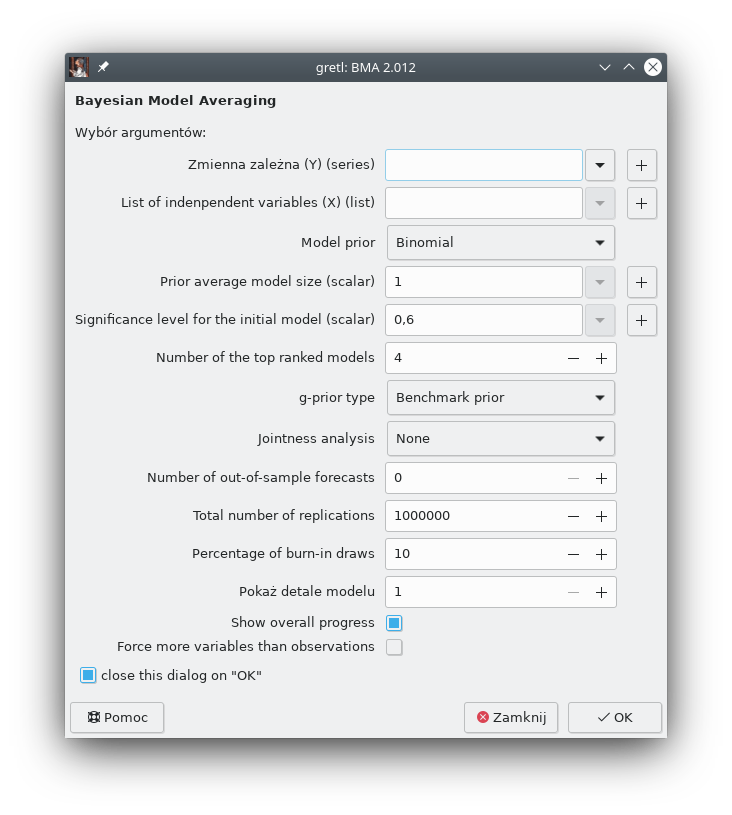
\includegraphics[width=0.7\columnwidth, keepaspectratio]{bma_main_window}
  \caption{Main window for \pkg{BMA}.}
  \label{fig:Main window for BMA}
\end{figure}
  
According to Figure~\ref{fig:Main window for BMA}, we can specify the following
entries in the GUI \pkg{BMA} window\label{text:module_parameters}
\begin{itemize}
\item \textbf{Dependent variable} -- The dependent variable.
\item \textbf{List of indenpendent variables}
  -- Loading variables from the database, which must have been
  opened previously.  Note that by
  default we assume that you want to estimate an intercept; therefore,
  a constant is implicitly included in the list of the variables.
\item \textbf{Model prior} -- Indicates the choice of model prior. One
  can employ the binomial model prior or the binomial-beta model
  prior. Note that the uniform model prior is a special case of the
  binomial model prior. Therefore, in fact, our package allows for
  three types of priors.
\item \textbf{Prior average model size} -- Specifies the prior
  expected model size $\E(\Xi)$.  The expected model size may range
  from 0 to \textit{K}. The default value equals 1.  It is the
  smallest reasonable prior expected model size. It means that we
  penalize large models and we assign high probability to small ones
  following Occam's razor philosophy.

  Note that for the binomial model prior and with $\E(\Xi)=0.5K$ one
  can define the uniform prior on the model space. For example, for
  $K=10$ regressors we can define the uniform prior with
  $\E(\Xi)=5$. For $\E(\Xi) < 5$ we assign high probability to small
  models.  The smaller the prior expected model size $\E(\Xi)$, the
  less probable are larger models.
\item \textbf{Significance level for the initial model} -- Defines the
  significance level which is used to build the initial model. An
  explanatory variable enters the initial model if its $p$~value is
  less than the significance level. If the significance level equals
  1, the initial model will be randomly chosen (with equal
  probability) from all available models. Note that if all available
  explanatory variables enter the initial model, you will get the
  following \pkg{gretl} error message ``No independent variables were
  omitted''.
\item \textbf{Number of top ranked models} -- Specifies the number of
  best models for which detailed information is stored.
\item \textbf{g-prior type} -- One can choose between four Zellner's
  g-priors for the regression coefficients. Choices include: benchmark
  prior, unit information prior, risk inflation criterion, Hannan and
  Quinn prior, root of g-UIP.
\item \textbf{Jointness analysis} -- If \code{"None"} (the default),
  the jointness analysis is omitted. Alternatively, one can choose the
  jointness measures of \cite{LeySteel2007} or
  \cite{DoppelhoferWeeks2009}.
\item \textbf{Number of out-of-sample forecasts} -- Defines the total
  number of out-of-sample forecasts of the dependent variable.
\item \textbf{Total number of replications} -- Defines the total
  number of iteration draws to be sampled.
\item \textbf{Percentage of burn-in draws} -- Specifies the number of
  burn-in replications, calculated as the percentage of the total
  number of iteration draws.
\item \textbf{Verbosity} -- An integer value of 1 or 2; the default is
  1, which allows to see the basic Bayesian model averaging
  results. If Verbosity equals 2, a more detailed description of the
  analysis is provided (initial model, speed of convergence,
  estimation results for top ranked models).
\item \textbf{Show overall progress} -- The output is flushed every 10\%
  of MC$^3$ and the progress is printed. Note: this consumes a lot of CPU time.
\end{itemize}     

\subsubsection{Script}
The \pkg{BMA} package can also be used inside \proglang{Hansl} scripts.
A very minimal code could be as follows:
%
\begin{CodeChunk}
\begin{CodeInput}
open greene9_1.gdt
include BMA.gfn
set seed 1000000
list greene = capital labor nfirm

BMA_GUI(valadd, greene, 1, 1.5, 0.6, 4, 1, 0, 0, 10000, 10, 1)
\end{CodeInput}
\end{CodeChunk}
%
The above example consists of three blocks.

The first block defines just the opening of the so-called \code{greene9_1}
dataset, which is bundled in every standard \pkg{gretl}
installation. This dataset contains the cross-sectional data on the
manufacturing of transportation equipment presented in
\cite{greene_Econometric_A}%
\footnote{This dataset is also available at link
  \url{http://people.stern.nyu.edu/wgreene/Text/Edition7/TableF7-2.txt}.}
and it consists of the following variables: valadd -- output, capital
-- capital input, labor -- labor input and nfirm -- number of firms.

The second block is the definition of the \code{greene} list which
contains indenpendent variables available in the \code{greene9_1} dataset.

The third block contains the specification of the Bayesian model
averaging analysis: binomial model prior, prior average model size set
to $1.5$ (which means that we have the uniform model prior), significance
level for the initial model set to $0.6$, 4 top ranked models,
Benchmark g-prior, without jointness analysis, without out-of-sample
forecasts, 1000000 replications with 10\% burn-in draws basic output
(verbosity set to 1) and progress overall progress is printed..

Suppose we want to run the same analysis but following Occam's razor
philosophy.  The simplest way to do this, is to set the prior average
model size to 1.  The code would be as follows:
%
\begin{CodeChunk}
\begin{CodeInput}
BMA_GUI(valadd, greene, 1, 1, 0.6, 4, 1, 0, 0, 10000, 10, 1, 1)
\end{CodeInput}
\end{CodeChunk}
%
In this case, we penalize large models by assigning high probabilities
to small ones. Apart from the binomial model prior, we can use the
binomial-beta prior. To do this, we have to set the model prior to
2. The code would be as follows
%
\begin{CodeChunk}
\begin{CodeInput}
BMA_GUI(valadd, greene, 2, 1, 0.6, 4, 1, 0, 0, 10000, 10, 1, 1)
\end{CodeInput}
\end{CodeChunk}
%
Suppose we want to set the g-prior to risk inflation criterion, select
the uniform model prior, do jointness analysis with the Ley-Steel
measure, compute forecasts for 3 observations and print additional
information (verbosity set to 2). The code would then be as follows:
%
\begin{CodeChunk}
\begin{CodeInput}
BMA_GUI(valadd, greene, 1, 1.5, 0.6, 4, 3, 1, 3, 10000, 10, 2, 0)
\end{CodeInput}
\end{CodeChunk}
%
Finally, if we want to save results of the above Bayesian model averaging analysis in
the the bundle \code{results_b}, the code should be as follows
%
\begin{CodeChunk}
\begin{CodeInput}
results_b = BMA_GUI(valadd, greene, 1, 1.5, 0.6, 4, 3, 1, 3, 10000, 10, 2, 0)
\end{CodeInput}
\end{CodeChunk}
%
Suppose we want to compute Doppelhofer-Weeks Measure instead of
already computed Ley-Steel Measure. Since the type of jointness measure
is controlled by 'do\_joint' field in the result bundle, the only thing
we have to do is to set the value of 'do\_join' to 2 and print BMA
results again. The code should be as follows:

\begin{CodeChunk}
\begin{CodeInput}
results_b.do_joint = 2
BMA_Print(&results_b)
\end{CodeInput}
\end{CodeChunk}
%
If we need backwards compatibility with BMA\_package prior to version 2
we can use the BMA\_OldStyle function to run the old style script.

\begin{CodeChunk}
\begin{CodeInput}
list greene_old = valadd capital labor nfirm
BMA_OldStyle(greene_old, 1, 1.5, 0.6, 4, 1, 1, 3, 10000, 10, 2)
\end{CodeInput}
\end{CodeChunk}

\subsubsection{Outputs}\label{sec:outputs}
If you select the appropriate entries in the GUI \pkg{BMA} window, our
package returns: PIP, Mean, Std.Dev., Cond.Mean, Cond.Std.Dev.
Furthermore, the package also returns the predictive results of the
dependent variable (Mean and Std.Dev.).

Let us consider the data used in \cite{FernandezLeySteel2001b}
(denoted FLS hereafter). This data comprises the information about 72
countries and 41 potential growth determinants for the period 1960 to
1992%
\footnote{The dataset is publicly available on the \emph{Journal of
    Applied Econometrics} online data archive
  (\url{http://qed.econ.queensu.ca/jae/2001-v16.5/fernandez-ley-steel/}).
  The reported chain (3000000 replications with 33\% burn-in draws)
  took about 51 minutes of CPU time on a PC with AMD Phenom II X6
  1100T CPU, 6.0~Gb of RAM running under Debian GNU/Linux. We used
  \pkg{gretl}~1.10.2 compiled by GCC~5.2.1. The seed for RNG was set
  to 1000000. The dependent variable is the growth rate from
  1960--1992.}. The initial estimation sample consists of indices
$i=1,\ldots,69$ and the out-of-sample evaluation indices are from 70
to 72.

For example, for the FLS data, the following estimates should appear
%
\begin{CodeChunk}
\begin{CodeOutput}
Posterior moments (unconditional and conditional on inclusion):
		   PIP         Mean     Std.Dev.    Cond.Mean   Cond.Std.Dev        
   GDPsh560   0.998378    -1.444579     0.305391    -1.446927       0.300031
Confuncious   0.890878     0.427081     0.189631     0.479393       0.123638
   Life_Exp   0.932297     0.988063     0.404005     1.059816       0.314688
  Equip_Inv   0.904971     0.549653     0.250217     0.607370       0.184734
  SubSahara   0.654270    -0.431560     0.369153    -0.659606       0.240550
     Muslim   0.363769     0.130498     0.197138     0.358739       0.157977
Rule_of_Law   0.416318     0.206002     0.271416     0.494818       0.184491
   Yrs_Open   0.547074     0.312026     0.318952     0.570354       0.196508
        ...        ...          ...          ...          ...            ...
----------------------------------
Posterior probability of models:
Model 1:    0.007899
Model 2:    0.005294
Model 3:    0.004204
Model 4:    0.003960
Model 5:    0.003378
     ...         ...
Total probability of the models in ranking (numerical): 0.058997
Correlation coefficient between the analytical
and numerical probabilities of the above models: 0.997518
----------------------------------
Predictive results:
            Growth       Mean   Std.Dev.
Obs.70    2.714600   1.590657   1.279354
Obs.71    2.067600   2.006087   0.941517
Obs.72    1.889700   2.465582   0.981258
\end{CodeOutput}
\end{CodeChunk}
%
The \pkg{BMA} estimate function accepts a scalar, which sets the verbosity
of the output. Its default value is 1, which causes the estimation
output to be printed out. A value of 2 forces the \pkg{BMA} function to
print out all the details of the estimation. You can print out the
above-mentioned results and additionally the following information:
the total CPU time, type of model prior, prior average model size,
significance level for the initial model, type of g-prior, total
number of iterations and, finally, the number of burn-in
draws. Moreover, the \pkg{BMA} estimate function produces the estimation
results for the initial and top ranked models. The jointness analysis
is inactive by default. If it is active, you will get: posterior joint
probability of explanatory variables, jointness statistic as given in
Equations~\ref{LS_jointness} or~\ref{DW_jointness} and classification
of jointness measures.  The jointness analysis for the previous
example should look like this:
%
\begin{CodeChunk}
\begin{CodeOutput}
Posterior joint probability of variables:
              GDPsh560 Confuncious   Life_Exp  Equip_Inv ...  
   GDPsh560   0.000000    0.889256   0.932182   0.903349 ...
Confuncious   0.000000    0.000000   0.826208   0.816956 ...
   Life_Exp   0.000000    0.000000   0.000000   0.839068 ...
  Equip_Inv   0.000000    0.000000   0.000000   0.000000 ...
        ...        ...         ...        ...        ... ...
Jointness statistics (Ley-Steel Measure):
              GDPsh560 Confuncious   Life_Exp  Equip_Inv ...
   GDPsh560   0.000000    2.083161   2.643181   2.235000 ...
Confuncious   0.000000    0.000000   1.576599   1.618373 ...
   Life_Exp   0.000000    0.000000   0.000000   1.662559 ...
  Equip_Inv   0.000000    0.000000   0.000000   0.000000 ...  
        ...        ...         ...        ...        ... ... 
Strong substitutes:
        Rev_Coup,Area       -4.516140
Rev_Coup,Publ_Edu_pct       -4.459739
                  ...             ...
Significant substitutes:   
       GDPsh560,Hindu       -1.997989
     Mining,War_Dummy       -1.989541
                  ...             ...   
Significant complements:
 Confuncious,Life_Exp        1.576599
Confuncious,Equip_Inv        1.618373
                  ...             ...
Strong complements:   
  DPsh560,Confuncious        2.083161
   GDPsh560,Equip_Inv        2.235000
                  ...             ...  
\end{CodeOutput}
\end{CodeChunk}
%
%%%%%%%%%%%%%%%%%%%%%%%%%%%%%%%%%%%%%%%%%%%%%%%%%%%%%%%%%%%%%%%%%%%%%%%%
\section{Comparison to other BMA software packages}\label{BmaGretlSec4}
Several Bayesian model averaging software packages have been developed by many
researchers%
\footnote{Useful information about Bayesian model averaging software
  packages are available at link
  \url{http://bms.zeugner.eu/resources/}.}.  The most popular in the
literature are \proglang{R} packages.  A recent and comprehensive overview of
Bayesian model averaging software in \proglang{R} is given in
\cite{AminiParmeter2011}. They outline the following BMA packages:
\pkg{BMS} by \cite{Zeugner_BMS}, \pkg{BAS} by
\cite{ClydeLittmanGhosh_BAS} and \pkg{BMA} by
\cite{RafteryHoetingVolinskyPainterYeung_BMA}.  According to their
research the \pkg{BMS} package provides the most accurate results and
it is also the most flexible with numerous options.
Table~\ref{tab:features_BMA_software} presents the main features of
the above mentioned packages.  Furthermore we compare our \pkg{BMA} package
to the \pkg{FLSBMA} program developed in \proglang{Fortran~77} by
\cite{FernandezLeySteel2001b}.

\begin{table}[t!]
 \centering
 \begin{tabular}{@{\extracolsep{-1pt}}lccccc}\hline
  Main features			&\proglang{R}-\pkg{BMS}			& \proglang{R}-\pkg{BMA}		& \proglang{R}-\pkg{BAS}	    &\pkg{FLSBMA}	      &\pkg{gretl}-\pkg{BMA}\\\hline
  \\[-10pt]
  \multirow{2}{*}{Model sampling}&\multirow{2}{*}{$\mbox{MC}^3$}		&\multirow{2}{*}{BIC}	&BAS, AMCMC,	    &\multirow{2}{*}{$\mbox{MC}^3$}     &\multirow{2}{*}{$\mbox{MC}^3$}\\
				&				&			&BAS+MCMC	    &			      &\\  
  Model priors			&5				&1			&3		    &2			      &3\\
  Zellner's g-priors	 	&6				&1			&9		    &9			      &5\\
  Jointness analysis	 	&				&			&		    &\checkmark		      &\checkmark\\
  Jointness measures     	&				&			&		    &1			      &2\\
  Out-of-sample forecast 	&\checkmark			&			&\checkmark         &\checkmark		      &\checkmark\\
  No.\ of burn-in draws		&\checkmark			&			&\checkmark         &\checkmark		      &\checkmark\\
  No.\ of draws	 		&\checkmark			&\checkmark		&\checkmark         &\checkmark		      &\checkmark\\
  No.\ of top ranked models  	&\checkmark			&			&	            &\checkmark		      &\checkmark\\
  Graphical user interface	&				&			&		    &			      &\checkmark\\\hline
 \end{tabular}
 \caption{Main features of the selected Bayesian model averaging software packages.
  Model sampling: Type of model sampling algorithms.
  Model priors: Number of available model priors.
  Zellner's g-priors: Number of available Zellner's factors of proportionality.
  Jointness analysis: Information if the package provides jointness analysis.
  Jointness measures: Number of available jointness measures.
  Out-of-sample forecast: Information about which package can be used for out-of-sample forecasting.
  No.~of burn-in draws.
  No.~of draws and no.~of top ranked models: Number of user-defined parameters in the sampling algorithm.
  Graphical user interface: Presence of a GUI in the package.}
 \label{tab:features_BMA_software}
\end{table}

The most flexible package according to the model sampling category is
\proglang{R}-\pkg{BAS} which contains three sampling algorithms: Bayesian
adaptive sampling (BAS), adaptive MCMC (AMCMC) and Bayesian adaptive
sampling with MCMC for the initial replications (BAS+MCMC).  All
packages offer different model priors. The most limited is
\proglang{R}-\pkg{BMA} with only a fixed model prior, while the most
comprehensive is \proglang{R}-\pkg{BMS} which contains the following model
priors: fixed, uniform, binomial, binomial-beta and custom
(user-controlled prior probabilities).  Furthermore, the number of
g-priors may differ depending on the package starting from one for
\proglang{R}-\pkg{BMA}, to nine for \proglang{R}-\pkg{BAS} and \pkg{FLSBMA}.

\pkg{gretl}-\pkg{BMA} and \pkg{FLSBMA} are the only packages which offer
Bayesian model averaging together with accompanying jointness
statistics.  \pkg{FLSBMA} contains one jointness measure (Ley-Steel)
while \pkg{gretl}-\pkg{BMA} contains two measures (Ley-Steel and
Doppelhofer-Weeks). The estimation of out-of-sample forecasts is
possible in almost all packages excluding \proglang{R}-\pkg{BMA}, where this
option is not available.  Three out of five packages enable full
control of the replication algorithm.  In \proglang{R}-\pkg{BMS}, \pkg{FLSBMA}
and \pkg{gretl}-\pkg{BMA}, the user can set the number of burn-in draws,
replication draws and detailed information about top ranked models.
Unlike other packages \pkg{gretl}-\pkg{BMA} offers an easy-to-use GUI for
the Bayesian model averaging approach.

In order to compare run times of the above mentioned packages we used
the FLS dataset with the following options: benchmark g-prior, 1000000
burn-in draws, 2000000 iterations.  Model prior was set to uniform. We
considered two scenarios for our experiment: with or without jointness
analysis.

\begin{table}[t!]
 \centering
 \begin{tabular}{lccccc}\hline
  Run time &\proglang{R}-\pkg{BMS} &\proglang{R}-\pkg{BMA} &\proglang{R}-\pkg{BAS} &\pkg{FLSBMA} &\pkg{gretl}-\pkg{BMA}\\\hline
  \\[-10pt]
  Without jointness analysis &317 &92 &53 &1423 &1852\\
  With jointness analysis 	&	&	&	&1423 &3073\\\hline  
 \end{tabular} 
 \caption{Run time in seconds of Bayesian model averaging software packages for FLS data.}
 \label{tab:FLS_packages_timings}
\end{table}

According to the results presented in
Table~\ref{tab:FLS_packages_timings}, the fastest Bayesian model
averaging software package is \proglang{R}-\pkg{BAS}, while the slowest one is
\pkg{gretl}-\pkg{BMA}. We are aware of this disadvantage of our package, but
it strongly depends on the \pkg{gretl} development process, especially on
the improvements of the \proglang{Hansl} interpreter. It is possible that in the
near future \pkg{gretl} will be much faster than the current 1.10.2
version (see Section~\ref{Conclusions} for more details).

%%%%%%%%%%%%%%%%%%%%%%%%%%%%%%%%%%%%%%%%%%%%%%%%%%%%%%%%%%%%%%%%%%%%%%%%%%%%%%%%%%%%%%%%
\section{Empirical illustration}\label{BmaGretlSec5}

\begin{sidewaystable}
\centering
  \begin{tabular}{lrrrrrrrrrr}\hline
    &\multicolumn{2}{c}{\proglang{R}-\pkg{BMS}}&\multicolumn{2}{c}{\proglang{R}-\pkg{BMA}}&\multicolumn{2}{c}{\proglang{R}-\pkg{BAS}}&\multicolumn{2}{c}{\pkg{FLSBMA}}&\multicolumn{2}{c}{\pkg{gretl}-\pkg{BMA}}\\\cline{2-11} 
    Regressors 		&Mean		&SD   	       &Mean	     &SD	     &Mean  & SD   &Mean	  &SD&Mean	  &SD\\ \hline
    Log GDP in 1960 	&$-1.425$ 	&0.280	       &$-1.595$	&0.195	&$-1.467$ &0.241 &$-1.418$& 0.267&$-1.427$	  &0.275\\
    Fraction Confucian  &\textbf{0.494} &0.127	       &0.641	&0.089	&0.579	&0.103 &0.490 & 0.117&\textbf{0.494}&0.126\\
    Life expectancy  	&0.954  	&0.396	       &1.024	&0.213	&1.004	&0.242 &0.958 & 0.370&0.967	  &0.386\\
    Equipment investment&0.553		&0.237	       &0.510	&0.121	&0.455	&0.164 &0.557 & 0.222&0.550&0.234\\
    Sub-Saharan dummy  	&$-0.472$ 	&0.346	       &$-0.919$	&0.172	&$-0.848$&0.214 &$-0.476$& 0.334&$-0.474$  &0.346\\
    Fraction Muslim  	&0.260 &0.228&0.149	&0.156	&0.141	&0.198  &0.257 & 0.219&0.261 &0.229\\
    \ldots & \multicolumn{10}{c}{\ldots}\\
    Population growth  	&\textbf{0.005}	&\textbf{0.048}&$-0.004$	&0.037	&0.006	&0.060 &0.003 & 0.035&\textbf{0.005}&\textbf{0.048}\\    
    British colony dummy  &$\mathbf{-0.003}$&\textbf{0.031}&0.360	 &0.133	&0.159		&0.196 &$-0.002$& 0.022&$\mathbf{-0.003}$&\textbf{0.031}\\
    Outward orientation   &$-0.003$&0.029	 &$-0.160$ &0.099	&$-0.074$	&0.102 &$-0.002$& 0.021&$-0.004$&0.030\\
    Fraction Jewish  	  &$\mathbf{-0.002}$&\textbf{0.027}&-0.001	 &0.010	&0.000	&0.022 &$-0.001$& 0.020&$\mathbf{-0.002}$&\textbf{0.027}\\
    Revolutions and coups &\textbf{0.000} &\textbf{0.023}&n/a	 &n/a	&\textbf{0.000}&0.024 &\textbf{0.000}	& 0.017&\textbf{0.000} &\textbf{0.023}\\
    Public education share&\textbf{0.001} &\textbf{0.023}&0.014	 &0.053	&0.061	&0.109 &0.000	& 0.017&\textbf{0.001} &\textbf{0.023}\\
    Area (scale effect)   &$\mathbf{-0.001}$&\textbf{0.021}&n/a	 &n/a	&$-0.003$&0.030 &$\mathbf{-0.001}$&0.014 &$\mathbf{-0.001}$&\textbf{0.021}\\\hline
  \end{tabular}
  \caption{The posterior estimates of regression coefficients based on
    the Bayesian model averaging software packages for the FLS data.
    The dependent variable is the growth rate from 1960--1992 across
    72 countries. All the regressors have been centered to have zero
    mean. Abbreviation ``n/a'' means that \proglang{R}-\pkg{BMA} dropped
    variable in pre-selection procedure.  Bold font denotes identical
    results.}
  \label{tab:Estimates of coefficients based on Bayesian model averaging}
\end{sidewaystable}


In this section we examine the ability of our package in replicating
the results published by \cite{FernandezLeySteel2001b} and
\cite{LeySteel2007}.  We use the same original dataset to attempt to
replicate their results. In our empirical illustration, we discard the
first 1 million models and draw samples from the model space 2 million
times. We specify the following entries in the GUI \pkg{BMA} window: model
prior = `binomial', prior average model size = `20.5' (we set the
model prior to the uniform distribution), number of the top ranked
models = `20', g-prior type = `Benchmark prior', total number of
replications = `3000000', percentage of burn-in draws = `33'.
Tables~\ref{tab:Estimates of coefficients based on Bayesian model
  averaging} and~\ref{tab:PIPs based on Bayesian model averaging}
present the estimation results%
\footnote{The reported chain took about 31 minutes of CPU time on a PC
  with AMD Phenom II X6 1100T CPU, 6.0~Gb of RAM running under Debian
  GNU/Linux. We used \pkg{gretl} 1.10.2 compiled by GCC~5.2.1. The
  seed for RNG was set to 1000000.}.  They report the posterior means,
standard errors and PIPs of regressors calculated by \proglang{R}-\pkg{BMS},
\proglang{R}-\pkg{BMA}, \proglang{R}-\pkg{BAS} and \pkg{FLSBMA} packages. These
benchmarking results allow us to compare and analyze the performance
of our package. Bold font indicates identical results.

As is apparent in Tables~\ref{tab:Estimates of coefficients based on
  Bayesian model averaging} and~\ref{tab:PIPs based on Bayesian model
  averaging}, the only minor differences in the posterior results are
found between \pkg{gretl}-\pkg{BMA} and the results published in
\cite{LeySteel2007}.  All PIPs and estimated posterior means or
standard deviations are reasonably close in all cases and the same
variables are identified to be relevant. Note that the \pkg{gretl} package
results are almost identical to the results produced by the
\proglang{R}-\pkg{BMS} package.

\begin{table}[t!]
\centering
  \begin{tabular}{lrrrrr}\hline
    Regressors 		  &\proglang{R}-\pkg{BMS}	&\proglang{R}-\pkg{BMA}	&\proglang{R}-\pkg{BAS}   &\pkg{FLSBMA}	&\pkg{gretl}-\pkg{BMA}\\\hline
    Log GDP in 1960 	  &\textbf{1.00}&\textbf{1.00}	&\textbf{1.00}	&\textbf{1.00}	&\textbf{1.00}\\
    Fraction Confucian    &\textbf{0.99}&	1.00	&	1.00	&	1.00	&\textbf{0.99}\\
    Life expectancy  	  &	0.93	&	1.00	&	1.00	&	0.95	&	0.94	\\
    Equipment investment  &\textbf{0.92}&	1.00	&	0.97	&	0.94	&\textbf{0.92}\\
    Sub-Saharan dummy  	  &\textbf{0.74}&	1.00	&	1.00	&	0.76	&\textbf{0.74}\\
    Fraction Muslim  	  &\textbf{0.65}&	0.60	&	0.43	&	0.66	&\textbf{0.65}\\
    \ldots & \multicolumn{5}{c}{\ldots}\\
    Population growth  	  &\textbf{0.04}&\textbf{0.04}	&	0.09	&	0.02	&\textbf{0.04}\\    
    British colony dummy  &\textbf{0.04}&	0.98	&	0.49	&	0.02	&\textbf{0.04}\\
    Outward orientation   &\textbf{0.04}&	0.86	&	0.44	&	0.02	&\textbf{0.04}\\
    Fraction Jewish    	  &\textbf{0.04}&	0.01	&	0.06	&	0.02	&\textbf{0.04}\\
    Revolutions and coups &\textbf{0.03}&	n/a	&	0.06	&	0.02	&\textbf{0.03}\\
    Public education share&\textbf{0.03}&	0.10	&	0.32	&	0.02	&\textbf{0.03}\\
    Area (scale effect)   &\textbf{0.03}&	n/a	&	0.06	&	0.02	&\textbf{0.03}\\\hline
  \end{tabular}
  \caption{Posterior inclusion probabilities based on the Bayesian model averaging software packages for FLS data.
    Abbreviation ``n/a'' means that \proglang{R}-\pkg{BMA} dropped the variable in the pre-selection procedure.
    Bold font denotes identical results.}
  \label{tab:PIPs based on Bayesian model averaging}
\end{table}

In our opinion, the main reason for the very similar results produced
by \proglang{R}-\pkg{BMS} and \pkg{gretl}-\pkg{BMA} is the implementation of the same
RNG algorithm (the SIMD-oriented Fast Mersenne Twister), while
\pkg{FLSBMA} package uses an older RNG algorithm, i.e., ``ran2''
developed by L'Ecuyer.  The \proglang{R}-\pkg{BMA} and \proglang{R}-\pkg{BAS} packages are
not capable to reproduce our results (see~\citealt{AminiParmeter2011}
for additional information).



%%%%%%%%%%%%%%%%%%%%%%%%%%%%%%%%%%%%%%%%%%%%%%%%%%%%%%%%%%%%%%%%%%%%%%%%%%%%%%%%%%%%%%%%
\section{Conclusions}\label{Conclusions}
This paper has outlined a new software package that implements
Bayesian model averaging and jointness measures for \pkg{gretl}. Bayesian
model averaging is a straightforward and natural extension of standard
Bayesian analysis and it is a useful and popular alternative to other
variable selection procedures, especially for a large set of
regressors. Here we used \pkg{gretl}, which is a free, open-source
software for econometric analysis with an easy-to-use GUI. Our goal
was to familiarize potential users with the features and the different
options that our package has to offer. We described how our package
implements Bayesian model averaging, as well as the outputs that are
returned.

Recent trends in Bayesian model averaging still concern applications
in various areas of empirical research, i.e., economic growth (see
\citealt{RePEc:taf:regstd:v:48:y:2014:i:1:p:44-67},
\citealt{GazdaPuziak2012}), stock returns (see
\citealt{RePEc:cqe:wpaper:2914}), geography (see
\citealt{RePEc:eee:csdana:v:75:y:2014:i:c:p:227-238}) and many more.
One can also encounter new papers about theory of Bayesian model
averaging, for example: two-stage Bayesian model averaging (see
\citealt{RePEc:taf:emetrv:v:33:y:2014:i:1-4:p:122-151}) or comparison
of Bayesian model averaging to the weighted average least squares
method (see \citealt{RePEc:dgr:kubcen:2011082}).

The future development of the \pkg{BMA} package could be focused on two
main aspects: speed improvements and feature extensions. The first one
is strongly correlated with the \pkg{gretl} development process, especially
with work on improvements in speed of the \proglang{Hansl} interpreter. It is
possible that the interpreter will be rewritten in the near future to
achieve speed boost with backward compatibility.  The feature
extensions would concern two aspects: implementing new g-priors and
model priors.  In the literature we can find many types of g-priors
(see \citealt{FernandezLeySteel2001a}).  Moreover new model priors
could be also considered.  For instance,
\cite{RePEc:aea:aecrev:v:94:y:2004:i:4:p:813-835} proposed the
so-called fixed model prior.  These implementations would surely
improve the flexibility of the \pkg{BMA} package.

\section*{Acknowledgments}
First, we would like to thank Allin Cottrell and Riccardo ``Jack''
Lucchetti for making the \pkg{gretl} project possible. We are also grateful
for the helpful comments and suggestions of two referees and an
associate editor.

\bibliography{BMA}

\end{document}
